\section{Introduction}

\textbf{Goal of course} is to understand principles of user-centered design and being able to apply these to practice.
Learn about the basic notions of Computational Design in HCI context. \medskip


\textbf{Moore's Law} \smallskip

Computational power grows exponentionally. Transistor count doubles every two years. Also with RAM and pixel densities. 
However: Human capabilities stay stable.\medskip

\textbf{Good System design} Accounts for human capabilities, human error and exceptional circumstances. \medskip

\textbf{Human Computer Interaction} \smallskip

Concerned with design, evaluation and implementation of interactive computing systems for human use. \medskip


\begin{center}
	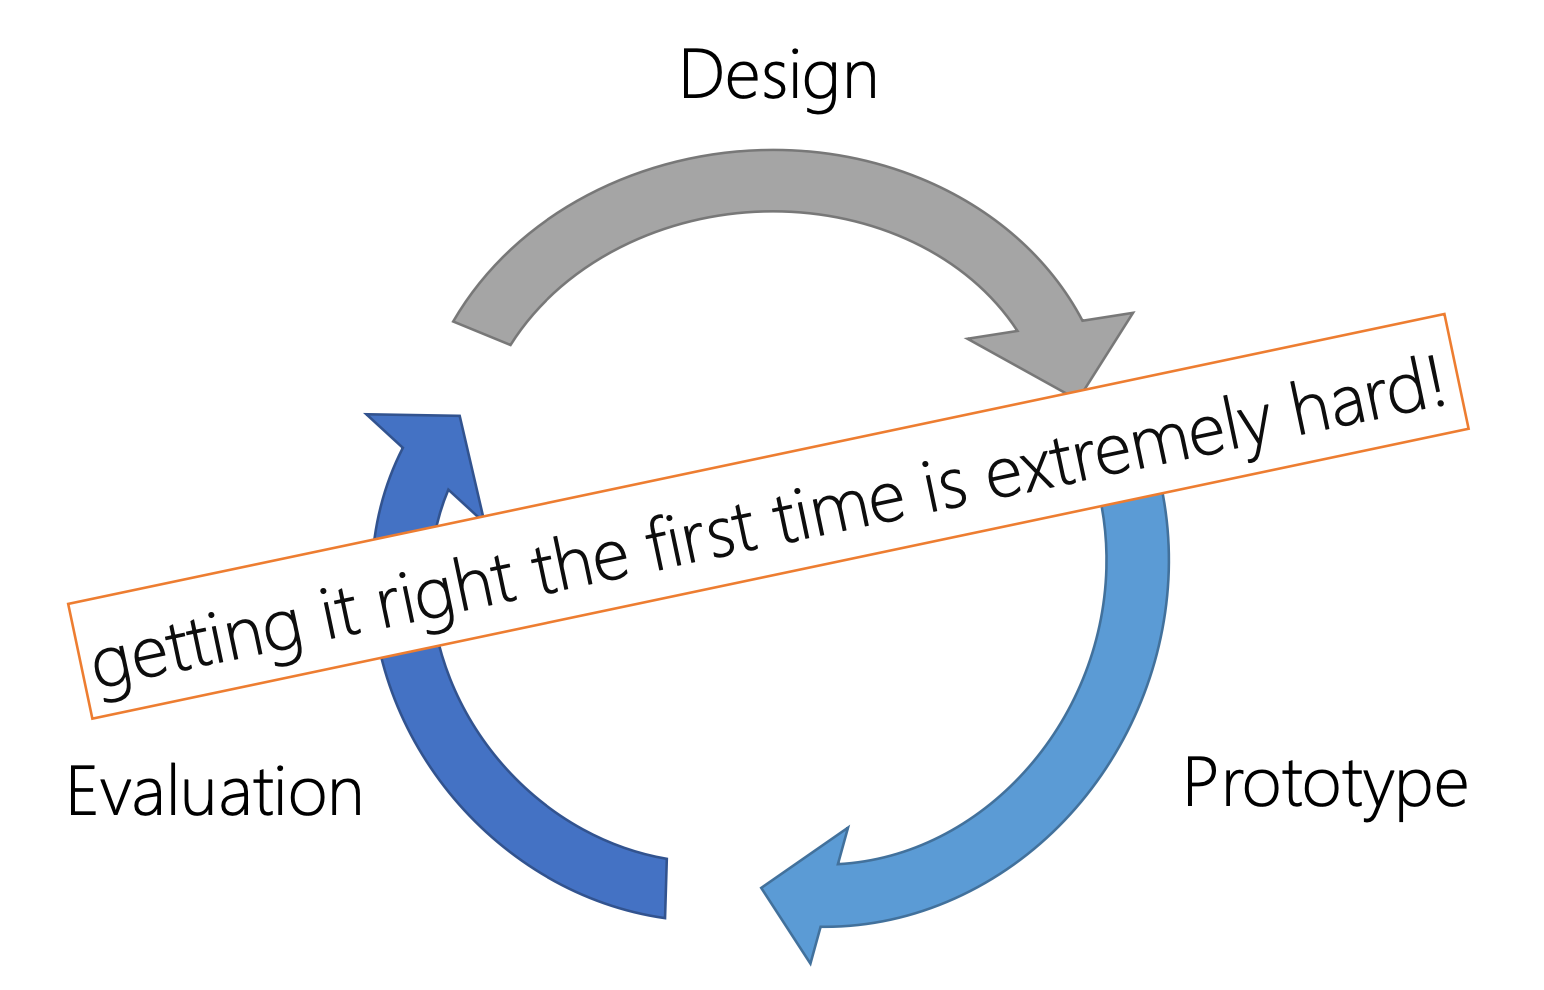
\includegraphics[width=\linewidth]{process.png}
\end{center}

\textit{Formative:} understand problem and user to inform our design. \medskip

\textit{Evaluative:} understand how well the design works. Also detects mistakes in design. \medskip

